\documentclass[10pt,xcolor=pst,aspectratio=169]{beamer}

\usepackage{etex}

%\usetheme{Boadilla}
%\usecolortheme{wolverine}
\usecolortheme{dolphin}
%\setbeamercovered{transparent}
%\setbeamercolor{block body}{bg=yellow}

\addtobeamertemplate{navigation symbols}{}{%
\usebeamerfont{footline}%
\usebeamercolor[fg]{footline}%
\hspace{1em}%
\insertframenumber/\inserttotalframenumber
}

\usepackage[utf8]{inputenc}
\usepackage[english,russian]{babel}
\usepackage[OT1]{fontenc}
\usepackage{amsmath, bm}
\usepackage{amsfonts}
\usepackage{amssymb}
\usepackage{graphicx}
\usepackage{wrapfig}
\usepackage[3D]{movie15}
\usepackage{animate}
\usepackage{ragged2e}
\usepackage{listings}
\usepackage{color}
\usepackage{pst-all}

\usepackage{tikz}
\usetikzlibrary{
    mindmap,
    arrows, % стрелки
    shapes.misc, % фигуры
    chains, % цепочки
    positioning, % позиционирование элементов
    scopes, % создание дополнительных веток
    shadows % тени
    }

\graphicspath{{pic/}}

\author{\textbf{Губкин А.С.}}

\title[Численные методы в физике]{Численные методы в физике}

\logo{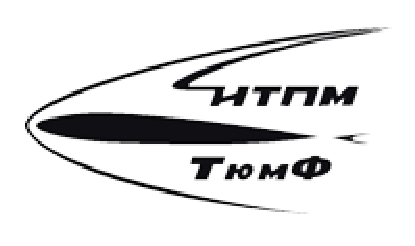
\includegraphics[width=0.1\linewidth]{LOGO_2.EPS}}

\institute[ТюмФ ИТПМ СО РАН]{Тюменский филиал Института теоретической и прикладной механики\\ им. С. А. Христиановича СО РАН, г. Тюмень}

%\date{6 октября 2015 г.}

\begin{document}

\lstset{ %
    language=[ANSI]C++,                 % выбор языка для подсветки (здесь это С++)
    keywordstyle=\color{blue},
    commentstyle=\color{gray},
    basicstyle=\scriptsize,
%basicstyle=\small\sffamily, % размер и начертание шрифта для подсветки кода
    numbers=left,               % где поставить нумерацию строк (слева\справа)
    numberstyle=\tiny,           % размер шрифта для номеров строк
%stepnumber=1,                   % размер шага между двумя номерами строк
    numbersep=4pt,                % как далеко отстоят номера строк от подсвечиваемого кода
%backgroundcolor=\color{white}, % цвет фона подсветки - используем \usepackage{color}
    showspaces=false,            % показывать или нет пробелы специальными отступами
    showstringspaces=false,      % показывать или нет пробелы в строках
    showtabs=false,             % показывать или нет табуляцию в строках
    frame=single,              % рисовать рамку вокруг кода
%tabsize=2,                 % размер табуляции по умолчанию равен 2 пробелам
    captionpos=t,              % позиция заголовка вверху [t] или внизу [b] 
    breaklines=true,           % автоматически переносить строки (да\нет)
    breakatwhitespace=true, % переносить строки только если есть пробел
    escapeinside={\%*}{*)}   % если нужно добавить комментарии в коде
}

%SLIDE #1
\begin{frame}

    \transdissolve[duration=0.1]
    \titlepage

\end{frame}

%SLIDE #
\begin{frame}{Введение}

    \transdissolve[duration=0.1]
    \justifying
    \large

    Законы сохранения первоначально возникают в интегральной форме, так как прямой физический смысл имеет функция множества, а не точки. Однако в классе гладких функций интегральная форма эквивалентна дифференциальным уравнениям поля. 

\end{frame}

%SLIDE #
\begin{frame}{Функции множества}

    \transdissolve[duration=0.1]
    \justifying
    \large

    \[
        \int^{x_{2}}_{x_{1}} f \left( x \right) dx
        =
        F \left( x_{2} \right)
        - F \left( x_{1} \right)
    \]

    \[
        \int^{2}_{1} x dx
        =
        \frac{1}{2} 2^{2}
        - \frac{1}{2} 1^{2}
        =
        \frac{3}{2}
    \]

    \[
        \int^{3}_{1} x dx
        =
        \frac{1}{2} 3^{2}
        - \frac{1}{2} 1^{2}
        =
        4
    \]

\end{frame}

%SLIDE #
\begin{frame}{Законы сохранения и уравнения поля}

    \transdissolve[duration=0.1]
    \justifying
    \large

    \[
        \left[ \int_{\Omega} \mathbf{s} \left( \mathbf{x}, t \right) d \mathbf{x} \right]^{t_{2}}_{t_{1}}
        + \int^{t_{2}}_{t_{1}} \oint_{\partial \Omega} \mathbf{A} \left( \mathbf{x}, t \right) \mathbf{n} d S d t
        + \int^{t_{2}}_{t_{1}} \oint_{\partial \Omega} \mathbf{g} \left( \mathbf{x}, t \right) d \mathbf{x} d t
        =
        0.
    \]

    \[
        \mathbf{x}
        =
        \left[
            \begin{split}
                &x_{1}\\
                &x_{2}\\
                &\vdots\\
                &x_{m}
            \end{split}
        \right], \;
        \mathbf{s}
        =
        \left[
            \begin{split}
                &s_{1}\\
                &s_{2}\\
                &\vdots\\
                &s_{m}
            \end{split}
        \right], \;
        \mathbf{g}
        =
        \left[
            \begin{split}
                &g_{1}\\
                &g_{2}\\
                &\vdots\\
                &g_{m}
            \end{split}
        \right], \;
        \mathbf{A}
        =
        \begin{bmatrix} 
            a_{11} & a_{12} & \ldots & a_{1n} \\
            a_{21} & a_{22} & \ldots & a_{2n} \\
            \vdots & \vdots & \ddots & \vdots \\
            a_{m1} & a_{m2} & \ldots & a_{mn} \\
        \end{bmatrix}.
    \]

\end{frame}

%SLIDE #
\begin{frame}{Законы сохранения и уравнения поля}

    \transdissolve[duration=0.1]
    \justifying
    \large

    Это уравнение утверждает, что изменение функции множества

    \[
        \bm{\Sigma} \left( \Omega, t \right) = \int_{\Omega} \mathbf{s}_{t} \left( \mathbf{x}, t \right) d \mathbf{x}
    \]

    на интервале времени от $t_{1}$ до $t_{2}$ уравновешено потоком величины $\mathbf{A}$ через $\partial \Omega$ и действием источников $\mathbf{g} \left( \mathbf{x}, t \right)$ в области $\Omega$ в течение того же времени. В основе физики сплошных сред, типичные компоненты функции $\Pi$ -- это масса, импульс, момент импульса, энергия, электрический заряд и т. д.

\end{frame}

%SLIDE #
\begin{frame}{Законы сохранения и уравнения поля}

    \transdissolve[duration=0.1]
    \justifying
    \large

    Законы сохранения дополняются исходными предположениями, которые определяют природу среды. Состояние системы описывается вектором состояния $\mathbf{u}$, так что величины $\mathbf{s}$, $\mathbf{g}$ и $\mathbf{A}$ зависят от $\mathbf{u}$ через известные дифференцируемые определяющие уравнения

    \[
        \mathbf{s}
    \]

%Основная задача состоит в том, чтобы найти векторное поле
%u(x, t), которое удовлетворяет уравнению A) для любых
%Q, tu t2 вместе с соответствующими начальными и граничными
%условиями.

\end{frame}

%SLIDE #
\begin{frame}{Система гиперболических законов сохранения}

    \transdissolve[duration=0.1]
    \justifying
    \large

    Системой гиперболических законов сохранения называется система вида:

    \[
        \vec{u}_{t} + \vec{\nabla} \cdot f \left( \vec{u} \right) = 0,
    \]

    где $u$ -- вектор сохраняемых величин, $f \left( \vec{u} \right)$ -- тензор потока.\\

    Такая запись уравнений в частных производных называется \textbf{консервативной} или \textbf{дивергентной}.\\

    Такие системы законов сохранения встречается в нефтянной отрасли, газовой динамике, теории мелкой воды и т.д.\\

\end{frame}

%SLIDE #
\begin{frame}{Уравнения Эйлера}

    \transdissolve[duration=0.1]
    \justifying
    \large

    Уравнения Эйлера можно представить в виде системы гиперболических законов сохранения:

%   \[
%       \begin{split}
%           &\frac{\partial \rho}{\partial t}
%               + \vec{\nabla} \cdot \rho \vec{v}
%               = 0, \\
%           &\frac{\partial \rho \vec{v}}{\partial t}
%               + \vec{\nabla} \cdot \left( \rho \vec{v} \vec{v} + p \textbf{I} \right)
%               =
%               \vec{F}, \\
%           &\frac{\partial \rho E}{\partial t}
%               + \vec{\nabla} \cdot \left( \vec{v} \left( \rho E + p \right) \right)
%               =
%               \vec{F} \cdot \vec{v},
%           \end{split}
%   \]

    \[
        \vec{u}_{t} + \vec{\nabla} \cdot f \left( \vec{u} \right) = \vec{q},
    \]

    \[
        \vec{u}
        =
        \begin{bmatrix}
            \rho \\
            \rho \vec{v} \\
            \rho E
        \end{bmatrix}, \:
        f (\vec{u})
        =
        \begin{bmatrix}
            \rho \vec{v} \\
            \rho \vec{v} \vec{v} + p \textbf{I}\\
            \vec{v}
            \left(
                \rho E + p
            \right)
        \end{bmatrix}, \:
        \vec{q}
        =
        \begin{bmatrix}
            0 \\
            \vec{F} \\
            \vec{F} \cdot \vec{v}
        \end{bmatrix}.
    \]

\end{frame}

%SLIDE #?
\begin{frame}{Одна особенность}

    \transdissolve[duration=0.1]
    \justifying
    \large

    Одной из особенностей нелинейных дифференциальных уравнений является то, что начальное условие, будучи гладким, может приводить к появлению разрывов в решении. Например ударные волны в газовой динамике.\\

\end{frame}

%SLIDE #?
\begin{frame}{Характеристики}

    \transdissolve[duration=0.1]
    \justifying
    \large
    
    Стандартным методом решения гиперболических уравнений является \textbf{метод характеристик}.\\

    Чтобы ввести понятие характеристики, перепишем скалярный гиперболический закон сохранения в \textbf{недивергентной} форме:

    \[
        u_{t} + f(u)_{x} = 0 \rightarrow \frac{\partial u}{\partial t} + \frac{\partial f}{\partial u} \frac{\partial u}{\partial x} = 0.
    \]

    Теперь, характеристиками будут линии в пространстве $(x, t)$, которые определяются с помощью уравнения:

    \[
        \frac{d x}{d t} = \frac{\partial f}{\partial u} = a(u).
    \]

\end{frame}

%SLIDE #?
\begin{frame}{Характеристики}

    \transdissolve[duration=0.1]
    \justifying
    \large

    Видно, что при таком определении $u$ будет константой вдоль характеристики, $u = u_{0}$:

    \[
        \begin{split}
            &u_{t} + f(u)_{x} = 0 \Rightarrow \frac{\partial u}{\partial t} + \frac{\partial f}{\partial u} \frac{\partial u}{\partial x} = 0 \Rightarrow \\
            &\Rightarrow \frac{\partial u}{\partial t} + \frac{d x}{d t} \frac{\partial u}{\partial x} = 0 \Rightarrow \frac{d u}{d t} = 0.
        \end{split}
    \]

\end{frame}

%SLIDE #?
\begin{frame}{Характеристики}

    \transdissolve[duration=0.1]
    \justifying
    \large

    Таким образом, уравнение характеристик будет иметь вид:

    \[
        \frac{d x}{d t} = a(u_{0}).
    \]

    Характеристики будут задаваться линиями:

    \[
        x(t) = a(u_{0}) (t - t_{0}) + x_{0}.
    \]

    \textbf{Значение переменной $u_0$ переносится вдоль этой линии.}

\end{frame}

%SLIDE #?
\begin{frame}{Метод характеристик}

    \transdissolve[duration=0.1]
    \justifying
    \large

    Пусть дана задача Коши для скалярного гипреболическооо уравнения:

    \[
        u_{t} + f(u)_{x} = 0, \: u(x) = \eta(x).
    \]

    Решение строится следующим образом: из произвольной точки $x_{0}$ на оси $x$ выпускаем характеристику. Коэффициент наклона характеристики, выходящей из точки $x_{0}$, есть $a_{0} = a(u_{0}) = a(u(x_{0}))$, так что уравнение характеристики: $x - x_{0} = a_{0} t$.\\

\end{frame}

%SLIDE #?
\begin{frame}{Метод характеристик}

    \transdissolve[duration=0.1]
    \justifying
    \large

    Таким образом, чтобы найти $u$ в точке $(x, t)$ следует определить характеристику, которая приходит в эту точку из точки $x_{0}$, из которой эта характеристика выходит, и так как $u_{0}$ постоянна на характеристике, то решение будет:

    \[
        u(x, t) = \eta(x_{0}) = \eta(x - a(u) t).
    \]

\end{frame}


%SLIDE #?
\begin{frame}{Метод характеристик}

    \transdissolve[duration=0.1]
    \justifying
    \large

    Такое построение решения не является удовлетворительным, так как характеристики могут пересекаться и по ним в одну и ту же точку будут переноситься различные значения $u$, так что решение становится многозначным. Чтобы устранить эту многозначность в решение вводят разрывы, на которых должны выполняться дополнительные условия.

\end{frame}

%SLIDE #?
\begin{frame}{Пример}

    \transdissolve[duration=0.1]
    \justifying
    \large

    Рассмотрим следующую задачу Коши для уравнения Бюргерса:

    \[
        \begin{cases}
            &u_{t} + \left( \frac{1}{2} u^{2} \right)_{x} = 0, \\
            &u(x, 0) = \sin (x), \quad - \infty < x < \infty.
        \end{cases}
    \]

\end{frame}

%SLIDE #?
\begin{frame}{Пример}

    \transdissolve[duration=0.1]
    \justifying
    \large

    В данном случае наклон характеристик есть

    \[
        a(u) = u.
    \]

    В начальный момент времени в точке $x = \pi / 2, \: u(\pi / 2) =~1$, тогда как в точке $x = 3 \pi / 2, \: u(3 \pi / 2) = - 1$.

\end{frame}

%SLIDE #?
\begin{frame}{Нарушение гладкости решения}

    \transdissolve[duration=0.1]
    \justifying
    \large

    \begin{center}
        \psset{xunit=1.8cm,yunit=1.8cm,algebraic=true}
        \begin{pspicture}(0,0)(6,3)
            \psgrid[griddots=20, gridwidth=0pt, gridcolor=gray, gridlabels=0pt, subgriddiv=1, subgriddots=20, subgridcolor=gray](0,0)(0,0)(6,3)
            \psaxes[Dx=3, Dy=3, subticks=1, labelFontSize=\scriptscriptstyle]{->}(0,0)(0,0)(6,3)[$x$,0][$t$,90]
            \psline[linewidth=2pt, linecolor=blue]{o->}(1.5707963,0)(3.1415926,1.5707963)
            \psline[linewidth=2pt, linecolor=red]{o->}(4.7123889,0)(3.1415926,1.5707963)
            \uput[-90](1.5707963,0){$u \left( \frac{\pi}{2} \right) = 1$}
            \uput[-90](4.7123889,0){$u \left( \frac{3 \pi}{2} \right) = - 1$}
            \uput[90](3.1415926,1.5707963){$u = ???$}
        \end{pspicture}
    \end{center}

\end{frame}

%SLIDE #?
\begin{frame}{Соотношения Рэнкина - Гюгонио}

    \transdissolve[duration=0.1]
    \justifying
    \large

    Рассмотрим разрыв решения. Пусть траектория движения разрыва суть $x(t)$, его скорость $s = x'(t) = \frac{d x}{d t}$, значение $u$ слева от разрыва обозначим $u_{L}$, справа от разрыва -- $u_{R}$. Интегральную форму закона сохранения

    \[
        \frac{d}{d t} \int_{a}^{b} u(x, t) dx = f(u(a, t)) - f(u(b, t)),
    \]

    можно переписать как

    \[
        \frac{d}{d t} \left( \int_{a}^{x(t)} u(x, t) dx + \int_{x(t)}^{b} u(x, t) dx \right) = f(u(a, t)) - f(u(b, t)).
    \]

\end{frame}

%SLIDE #?
\begin{frame}{Соотношения Рэнкина - Гюгонио}

    \transdissolve[duration=0.1]
    \justifying
    \large

    Выполняя дифференцирование, получаем

    \[
        \begin{split}
            &\int_{a}^{x(t)} u_{t} dx + u(x(t) - \varepsilon,t) x'(t) + \\
            &+ \int_{x(t)}^{b} u_{t} dx - u(x(t) + \varepsilon,t) x'(t)= \\
            &= f(u(a, t)) - f(u(b, t)).
        \end{split}
    \]

\end{frame}

%SLIDE #?
\begin{frame}{Соотношения Рэнкина - Гюгонио}

    \transdissolve[duration=0.1]
    \justifying
    \large

    Подставив $u_{t} = - f_{x}$ и выполняя интегрирование, получаем

    \[
        \begin{split}
            &f(u(t, a)) - f(u(t, x(t) - \varepsilon)) + u(t, x(t) - \varepsilon) x'(t) + \\
            &f(u(t, x(t) + \varepsilon)) - f(u(t, b)) - u(t, x(t) + \varepsilon ) x'(t) = \\
            &= f(u(t, a)) - f(u(t, b)).
        \end{split}
    \]

    Окончательно получаем

    \[
        s(u_{L} - u_{R}) = f(u_{L}) - f(u_{R}).
    \]

\end{frame}

%SLIDE #?
\begin{frame}{Обобщенное решение}

    \transdissolve[duration=0.1]
    \justifying
    \large

    Решение, содержащее разрывы, не является классическим в том смысле, что не имеет непрерывных производных по каждой из переменных. Решения такого типа называются \textbf{обобщенными}. Обобщенное решение задачи Коши для нелинейных уравнений не является единственным.

\end{frame}

%SLIDE #?
\begin{frame}{Пример}

    \transdissolve[duration=0.1]
    \justifying
    \large

    Сделанное утверждение проиллюстрируем следующим примером. Рассмотрим следующую задачу Коши:

    \[
        \begin{cases}
            &u_{t} + \left( \frac{1}{2} u^{2} \right)_{x} = 0, \\
            &u(x, 0) = \eta(x) =
            \begin{cases}
                &u_{L}, \quad x < 0, \\
                &u_{R}, \quad x > 0,
            \end{cases}
        \end{cases}
    \]

    причем $u_{L} < u_{R}$.

\end{frame}

%SLIDE #?
\begin{frame}{Два решения}

    \transdissolve[duration=0.1]
    \justifying
    \normalsize

    \vspace{-5ex}

    \begin{center}
        Можно указать два обобщенных решения этой задачи:
    \end{center}

    \vspace{-5ex}

    \begin{minipage}{0.45\textwidth}
        \begin{center}
            \[
                \begin{split}
                    &u(x, t) = \eta(x - s t), \\
                    &s = \frac{u_{L} + u_{R}}{2}.
                \end{split}
            \]
        \end{center}
    \end{minipage}
    \hfill
    \begin{minipage}{0.45\textwidth}
        \begin{center}
            \[
                u(x ,t) =
                \begin{cases}
                    &u_{L}, \: x < u_{L} t \\
                    &\frac{x}{t}, \: u_{L} t < x < u_{R} t \\
                    &u_{R}, \: x > u_{R} t.
                \end{cases}
            \]
        \end{center}
    \end{minipage}

    \begin{minipage}{0.45\textwidth}
        \begin{center}
            \psset{xunit=1.5cm,yunit=1.5cm,algebraic=true}
            \begin{pspicture}(0,0)(3,3)
                \psgrid[griddots=20, gridwidth=0pt, gridcolor=gray, gridlabels=0pt, subgriddiv=0, subgriddots=20, subgridcolor=gray](0,0)(3,3)
                \psaxes[Dx=5, Dy=5, subticks=0, labelFontSize=\scriptscriptstyle]{->}(0,0)(3,3)[$x$,0][$t$,90]

                \psplot[linewidth=2pt, linecolor=green, yMaxValue=3, yMinValue=0]{0}{3} {2*x + 2.5}
                \psplot[linewidth=2pt, linecolor=green, yMaxValue=3, yMinValue=0]{0}{3} {2*x + 2}
                \psplot[linewidth=2pt, linecolor=green, yMaxValue=3, yMinValue=0]{0}{3} {2*x + 1.5}
                \psplot[linewidth=2pt, linecolor=green, yMaxValue=3, yMinValue=0]{0}{3} {2*x + 1}
                \psplot[linewidth=2pt, linecolor=green, yMaxValue=3, yMinValue=0]{0}{3} {2*x + 0.5}
                \psplot[linewidth=2pt, linecolor=green, yMaxValue=3, yMinValue=0]{0}{3} {2*x}
                \psplot[linewidth=2pt, linecolor=green, yMaxValue=3, yMinValue=0]{0.5}{3} {2*x - 0.5}
                \psplot[linewidth=2pt, linecolor=green, yMaxValue=3, yMinValue=0]{1}{3} {2*x - 1}
                \psplot[linewidth=2pt, linecolor=green, yMaxValue=3, yMinValue=0]{1.5}{3} {2*x - 1.5}
                \psplot[linewidth=2pt, linecolor=green, yMaxValue=3, yMinValue=0]{2}{3} {2*x - 2}
                \psplot[linewidth=2pt, linecolor=green, yMaxValue=3, yMinValue=0]{2.5}{3} {2*x - 2.5}

                \psplot[linewidth=2pt, linecolor=blue, yMaxValue=3, yMinValue=0]{0}{3} {x}

                \psplot[linewidth=2pt, linecolor=red, yMaxValue=3, yMinValue=0]{2.4}{3} {0.5*x + 1.2}
                \psplot[linewidth=2pt, linecolor=red, yMaxValue=3, yMinValue=0]{1.8}{3} {0.5*x + 0.9}
                \psplot[linewidth=2pt, linecolor=red, yMaxValue=3, yMinValue=0]{1.2}{3} {0.5*x + 0.6}
                \psplot[linewidth=2pt, linecolor=red, yMaxValue=3, yMinValue=0]{0.6}{3} {0.5*x + 0.3}
                \psplot[linewidth=2pt, linecolor=red, yMaxValue=3, yMinValue=0]{0}{3} {0.5*x}
                \psplot[linewidth=2pt, linecolor=red, yMaxValue=3, yMinValue=0]{0}{3} {0.5*x - 0.3}
                \psplot[linewidth=2pt, linecolor=red, yMaxValue=3, yMinValue=0]{0}{3} {0.5*x - 0.6}
                \psplot[linewidth=2pt, linecolor=red, yMaxValue=3, yMinValue=0]{0}{3} {0.5*x - 0.9}
                \psplot[linewidth=2pt, linecolor=red, yMaxValue=3, yMinValue=0]{0}{3} {0.5*x - 1.2}
                \psplot[linewidth=2pt, linecolor=red, yMaxValue=3, yMinValue=0]{0}{3} {0.5*x - 1.5}
            \end{pspicture}
        \end{center}
    \end{minipage}
    \hfill
    \begin{minipage}{0.45\textwidth}
        \begin{center}
            \psset{xunit=1.5cm,yunit=1.5cm,algebraic=true}
            \begin{pspicture}(0,0)(3,3)
                \psgrid[griddots=20, gridwidth=0pt, gridcolor=gray, gridlabels=0pt, subgriddiv=0, subgriddots=20, subgridcolor=gray](0,0)(3,3)
                \psaxes[Dx=5, Dy=5, subticks=0, labelFontSize=\scriptscriptstyle]{->}(0,0)(3,3)[$x$,0][$t$,90]

                \psplot[linewidth=2pt, linecolor=green, yMaxValue=3, yMinValue=0]{0}{3} {2*x + 2.5}
                \psplot[linewidth=2pt, linecolor=green, yMaxValue=3, yMinValue=0]{0}{3} {2*x + 2}
                \psplot[linewidth=2pt, linecolor=green, yMaxValue=3, yMinValue=0]{0}{3} {2*x + 1.5}
                \psplot[linewidth=2pt, linecolor=green, yMaxValue=3, yMinValue=0]{0}{3} {2*x + 1}
                \psplot[linewidth=2pt, linecolor=green, yMaxValue=3, yMinValue=0]{0}{3} {2*x + 0.5}

                \psplot[linewidth=2pt, linecolor=blue, yMaxValue=3, yMinValue=0]{0}{3} {2*x}

                \psplot[linewidth=2pt, linecolor=yellow, yMaxValue=3, yMinValue=0]{0}{3} {1.7*x}
                \psplot[linewidth=2pt, linecolor=yellow, yMaxValue=3, yMinValue=0]{0}{3} {1.4*x}
                \psplot[linewidth=2pt, linecolor=yellow, yMaxValue=3, yMinValue=0]{0}{3} {1.1*x}
                \psplot[linewidth=2pt, linecolor=yellow, yMaxValue=3, yMinValue=0]{0}{3} {0.9*x}

                \psplot[linewidth=2pt, linecolor=blue, yMaxValue=3, yMinValue=0]{0}{3} {0.8*x}

                \psplot[linewidth=2pt, linecolor=red, yMaxValue=3, yMinValue=0]{0}{3} {0.8*x - 2.1}
                \psplot[linewidth=2pt, linecolor=red, yMaxValue=3, yMinValue=0]{0}{3} {0.8*x - 1.8}
                \psplot[linewidth=2pt, linecolor=red, yMaxValue=3, yMinValue=0]{0}{3} {0.8*x - 1.5}
                \psplot[linewidth=2pt, linecolor=red, yMaxValue=3, yMinValue=0]{0}{3} {0.8*x - 1.2}
                \psplot[linewidth=2pt, linecolor=red, yMaxValue=3, yMinValue=0]{0}{3} {0.8*x - 0.9}
                \psplot[linewidth=2pt, linecolor=red, yMaxValue=3, yMinValue=0]{0}{3} {0.8*x - 0.6}
                \psplot[linewidth=2pt, linecolor=red, yMaxValue=3, yMinValue=0]{0}{3} {0.8*x - 0.3}
            \end{pspicture}
        \end{center}
    \end{minipage}

\end{frame}

%SLIDE #?
\begin{frame}{Энтропийное условие}

    \transdissolve[duration=0.1]
    \justifying
    \large

    Чтобы выделить единственное решение, необходимо наложить на него дополнительные требования: \textbf{возрастание (убывание) энтропии на скачке}.\\

    \textbf{Энтропийное условие} указывает на то, что реализуется только то состояние, в котором характеристики входят в разрыв и не могут выходить из разрыва.\\

    Алгебраически энтропийное условие может быть записано следующим образом:

    \vspace{-2ex}

    \[
        a(u_{L}) = f'(u_{L}) \geq \frac{f(u_{R}) - f(u_{L})}{u_{R} - u_{L}} \geq f'(u_{R}) = a(u_{R}).
    \]

    %Т.е. наклон прямой, соединяющей точки $u_{L}$ и $u_{R}$, должен быть больше наклона касательной в точке $u_{R}$ и меньше чем в точке $u_{L}$.

\end{frame}

%SLIDE #?
\begin{frame}{Решение}

    \transdissolve[duration=0.1]
    \justifying
    \normalsize

    \vspace{-2ex}

    \begin{center}
        Таким образом, решением будет функция:
    \end{center}

    \vspace{-5ex}

    \begin{center}
        \[
            u(x ,t) =
            \begin{cases}
                &u_{L}, \: x < u_{L} t \\
                &\frac{x}{t}, \: u_{L} t < x < u_{R} t \\
                &u_{R}, \: x > u_{R} t.
            \end{cases}
        \]
    \end{center}

    \begin{center}
        \psset{xunit=1.5cm,yunit=1.5cm,algebraic=true}
        \begin{pspicture}(0,0)(3,3)
            \psgrid[griddots=20, gridwidth=0pt, gridcolor=gray, gridlabels=0pt, subgriddiv=0, subgriddots=20, subgridcolor=gray](0,0)(3,3)
            \psaxes[Dx=5, Dy=5, subticks=0, labelFontSize=\scriptscriptstyle]{->}(0,0)(3,3)[$x$,0][$t$,90]

            \psplot[linewidth=2pt, linecolor=green, yMaxValue=3, yMinValue=0]{0}{3} {2*x + 2.5}
            \psplot[linewidth=2pt, linecolor=green, yMaxValue=3, yMinValue=0]{0}{3} {2*x + 2}
            \psplot[linewidth=2pt, linecolor=green, yMaxValue=3, yMinValue=0]{0}{3} {2*x + 1.5}
            \psplot[linewidth=2pt, linecolor=green, yMaxValue=3, yMinValue=0]{0}{3} {2*x + 1}
            \psplot[linewidth=2pt, linecolor=green, yMaxValue=3, yMinValue=0]{0}{3} {2*x + 0.5}

            \psplot[linewidth=2pt, linecolor=blue, yMaxValue=3, yMinValue=0]{0}{3} {2*x}

            \psplot[linewidth=2pt, linecolor=yellow, yMaxValue=3, yMinValue=0]{0}{3} {1.7*x}
            \psplot[linewidth=2pt, linecolor=yellow, yMaxValue=3, yMinValue=0]{0}{3} {1.4*x}
            \psplot[linewidth=2pt, linecolor=yellow, yMaxValue=3, yMinValue=0]{0}{3} {1.1*x}
            \psplot[linewidth=2pt, linecolor=yellow, yMaxValue=3, yMinValue=0]{0}{3} {0.9*x}

            \psplot[linewidth=2pt, linecolor=blue, yMaxValue=3, yMinValue=0]{0}{3} {0.8*x}

            \psplot[linewidth=2pt, linecolor=red, yMaxValue=3, yMinValue=0]{0}{3} {0.8*x - 2.1}
            \psplot[linewidth=2pt, linecolor=red, yMaxValue=3, yMinValue=0]{0}{3} {0.8*x - 1.8}
            \psplot[linewidth=2pt, linecolor=red, yMaxValue=3, yMinValue=0]{0}{3} {0.8*x - 1.5}
            \psplot[linewidth=2pt, linecolor=red, yMaxValue=3, yMinValue=0]{0}{3} {0.8*x - 1.2}
            \psplot[linewidth=2pt, linecolor=red, yMaxValue=3, yMinValue=0]{0}{3} {0.8*x - 0.9}
            \psplot[linewidth=2pt, linecolor=red, yMaxValue=3, yMinValue=0]{0}{3} {0.8*x - 0.6}
            \psplot[linewidth=2pt, linecolor=red, yMaxValue=3, yMinValue=0]{0}{3} {0.8*x - 0.3}
        \end{pspicture}
    \end{center}

\end{frame}

%SLIDE #?
\begin{frame}{Энтропийное условие. Пояснение}

    \transdissolve[duration=0.1]
    \justifying
    \large

    Точка разрыва переменных есть идеализация, описывающая область резких градиентов решения. На самом деле в этой области становятся существенными слагаемые, которыми в областях гладкости можно пренебречь: часто они имеют диффузионный вид. С учетом этого замечания введем малую диффузию:

    \[
        u_{t} + f(u)_{x} = \left( \nu u_{x} \right)_{x}.
    \]

    Нас интересует предельное поведение решений этого уравнения при $\nu~\rightarrow~0$. Этот предел (если он существует) мы обьявляем решением уравнения без вязкости.

\end{frame}

%SLIDE #?
\begin{frame}{Энтропийное условие. Пояснение}

    \transdissolve[duration=0.1]
    \justifying
    \large

    Пусть $E(u)$ - произвольная функция, определенная при всех $u$. Умножим исходное уравнение на $E_{u}(u)$ и после несложных преобразований получим:

    \[
        \begin{split}
            &E_{u} u_{t} + E_{u} f(u)_{u} u_{x} = E_{u} \left( \nu u_{x} \right)_{x} \Rightarrow \\
            &\Rightarrow E_{t} + \frac{\partial}{\partial x} \int{E_{u} f_{u} du} = \left( \nu E_{u} u_{x} \right)_{x} - \nu E_{uu} \left( u_{x} \right)^{2}.
        \end{split}
    \]

\end{frame}

%SLIDE #?
\begin{frame}{Энтропийное условие. Пояснение}

    \transdissolve[duration=0.1]
    \justifying
    \large

    Интегрируя по $x$ от $-\infty$ до $\infty$, получаем

    \[
        \left. -s E \right|_{-\infty}^{\infty} + \left. \left( F - \nu E_{u} u_{x} \right) \right|_{-\infty}^{\infty} = -\int_{-\infty}^{\infty}{\nu E_{uu} \left( u_{x} \right)^{2} dx},
    \]

    где $F = \int{E_{u} f_{u} du}$ -- поток величины $E$.

\end{frame}

%SLIDE #?
\begin{frame}{Энтропийное условие. Пояснение}

    \transdissolve[duration=0.1]
    \justifying
    \large

    Вне разрыва член $\nu E_{u} u_{x} \rightarrow 0$ при $\nu \rightarrow 0$. Кроме того, $\left. (\cdot) \right|_{-\infty}^{\infty} = -[\cdot]$, так что последнее соотношение примет вид:

    \[
        -s [E] + [F] = -\int_{-\infty}^{\infty}{\nu E_{uu} \left( u_{x} \right)^{2} dx}.
    \]

\end{frame}

%SLIDE #?
\begin{frame}{Энтропийное условие. Пояснение}

    \transdissolve[duration=0.1]
    \justifying
    \large

    Если функция $E(u)$ такая, что $s_{uu} < 0$, то в пределе получаем неравенство

    \[
        -s [E] + [F] \leq 0.
    \]

    В этом случае $E(u)$ называется \textbf{энтропией}. Для скалярного уравнения таких функций существует бесконечно много.

\end{frame}

%SLIDE #?
\begin{frame}{Энтропийное условие. Пояснение}

    \transdissolve[duration=0.1]
    \justifying
    \large

    Смысл неравенства $s[E] \geq [F]$ следующий: скорость приращения энтропии $s[E]$ не меньше, чем ее подвод извне $[F]$. На разрывах за счет действия <<диссипативных>> процессов рост энтропии превышает ее подвод. Это обстоятельство можно записать так

    \[
        E_{t} + F_{x} \geq 0.
    \]

    Таким образом, на обобщенное решение уравнения можно наложить дополнительное условие \textbf{возрастания энтропии}.\\
    \textbf{Замечание:} если под энтропией понимать функцию, такую что $E_{uu} > 0$, то следует говорить об убывании энтропии на разрыве.

\end{frame}

\end{document}